% !TEX program = xelatex
% VDT 2026 report: the paper's content (iclr2025_conference.tex) in the style of
% "Biểu mẫu báo cáo VDT 2026.docx.doc": A4, margins 2 cm top and 1.5 cm elsewhere, a one-column
% title block, then two columns 0.5 cm apart in Times New Roman 13.5 pt, justified, with bold
% numbered upper-case section headings. At most 6 A4 pages.
% Build with XeLaTeX (system Times New Roman):  latexmk -xelatex vdt_report.tex
\documentclass[a4paper]{article}
\usepackage[a4paper, top=2cm, bottom=1.5cm, left=1.5cm, right=1.5cm, columnsep=0.5cm,
            footskip=0.75cm]{geometry}
\usepackage{fontspec}
\setmainfont{Times New Roman}
\usepackage{graphicx}
\usepackage{booktabs}
\usepackage{float}
\usepackage{url}
\usepackage[numbers, sort&compress]{natbib}
\usepackage[hidelinks]{hyperref}
\usepackage{enumitem}

% Body text: 13.5 pt on a 15.5 pt line, as in the template's Normal style.
\renewcommand{\normalsize}{\fontsize{13.5pt}{15.5pt}\selectfont}
\renewcommand{\small}{\fontsize{11pt}{13pt}\selectfont}
\renewcommand{\footnotesize}{\fontsize{10pt}{12pt}\selectfont}
\normalsize
\setlength{\parindent}{0pt}
% Narrow 13.5 pt columns: let lines stretch, as Word's justification does, instead of overflowing.
\sloppy
\setlength{\emergencystretch}{3em}
\setlength{\parskip}{2pt}
\setlist{nosep, leftmargin=1.2em}
\renewcommand{\labelitemi}{--}

% Headings as in Interspeech papers: numbered ("1."), bold; sections centred, subsections
% left-aligned.
\makeatletter
\renewcommand{\section}{\@startsection{section}{1}{0pt}{7pt}{7pt}{\normalfont\normalsize\bfseries\centering}}
\renewcommand{\subsection}{\@startsection{subsection}{2}{0pt}{5pt}{3pt}{\normalfont\normalsize\bfseries}}
\renewcommand{\@seccntformat}[1]{\csname the#1\endcsname.\hspace{0.6em}}
\makeatother
\renewcommand{\bibsection}{\section{References}}
\renewcommand{\bibfont}{\footnotesize}
\setlength{\bibsep}{0pt}

\usepackage{caption}
\captionsetup{font=small, labelfont=bf, skip=4pt}
\setlength{\textfloatsep}{8pt}
\setlength{\floatsep}{6pt}
\setlength{\dbltextfloatsep}{8pt}
% Let several full-width tables share the top of a page instead of one per float page.
\setcounter{dbltopnumber}{4}
\renewcommand{\dbltopfraction}{0.85}
\renewcommand{\dblfloatpagefraction}{0.8}

\newcommand{\viet}[1]{#1}

\begin{document}
\twocolumn[{%
  \centering
  \vspace*{12pt}
  {\fontsize{18pt}{22pt}\selectfont\bfseries Non-verbal Vocalization Control for\\
   Vietnamese Text-to-Speech\par}
  % TODO: final title.
  \vspace{16pt}
  {\fontsize{15pt}{18pt}\selectfont\itshape To Duy An, Nguyen Tung Luong$^{1}$, Tran Hong Nhat$^{1}$,
   Do Van Hai$^{1}$\par}
  \vspace{2pt}
  {\fontsize{15pt}{18pt}\selectfont\itshape $^{1}$Viettel AI\par}
  \vspace{1pt}
  {\fontsize{11pt}{13pt}\selectfont\ttfamily luongnt29@viettel.com.vn, nhatth2@viettel.com.vn,
   haidv21@viettel.com.vn\par}
  \vspace{16pt}
}]

{\centering\bfseries Abstract\par}
\vspace{3pt}
Text-to-speech (TTS) systems can read Vietnamese aloud, but
they cannot yet reliably make non-verbal sounds, such as laughing, sighing or coughing, at the
point where the text asks for them. These sounds make synthetic speech feel human in voice
assistants, customer-facing AI agents, audiobooks and videos. Two things stand in the way:
existing systems ignore or garble such tags in Vietnamese, and no Vietnamese training data with
labelled sounds exists. We build that data automatically by adapting the SynParaSpeech method
to Vietnamese: recordings of real sounds are converted into each speaker's voice and inserted
into natural pauses in real Vietnamese speech, with a matching tag in the transcript. The result
is about 811 hours of labelled speech covering 17 sound types. Fine-tuning the open-source
OmniVoice model on this data teaches it 15 new tags. The fine-tuned model makes the right sound
at the right place for 50\% of tags, against 11.5\% for the released model, and misses only 35\%
of them, against 64\%. Its word error rate on the tagged sentences falls from 8.1\% to 6.7\%; on
plain text it rises a little, from 3.9\% to 4.8\%, with the same speaker similarity, and it runs
at a real-time factor of 0.06, fast enough for live conversation.

\textbf{\textit{Index Terms}}: text-to-speech, non-verbal vocalization, paralinguistics,
Vietnamese, data synthesis

\section{Introduction}\label{sec:intro}
When people talk, they communicate with more than words. A short laugh, a sigh, a breath before
a long sentence or a hesitant ``ừm\ldots'' tells the listener how the speaker feels and what
they mean. These paralinguistic, or non-verbal, cues, which we call non-verbal vocalizations
(NVVs), run through everyday conversation, and speech without them sounds flat and mechanical
even when every word is pronounced correctly.

Text-to-speech (TTS) systems turn written text into spoken audio. Modern TTS models read text
clearly in many voices, and some now let the user place a tag in the text, as in ``Thật à
[laughter] mình không ngờ luôn'' (``Really? [laughter] I didn't expect that at all''), so that
the voice laughs at exactly that point. A voice agent that answers customers can then chuckle at
a joke or sigh in sympathy at a complaint, and that small reaction is often what makes a caller
feel heard rather than processed; an audiobook or a dubbed video can let its narrator gasp or
laugh where the script calls for it.

For Vietnamese, this control does not exist yet. What is needed is a TTS system that, given a
Vietnamese sentence with a tag such as [cough], makes that sound at that point in the sentence,
in the chosen voice, as naturally as a person would. To our knowledge, no available system can
do this. Fish Audio's open model, OpenAudio S1~\citep{openaudios1}, offers markers such as
(laughing) and (sighing) in 13 languages, none of them Vietnamese. OmniVoice~\citep{omnivoice}
does speak Vietnamese, but its tags were learned from Chinese and English data: in our tests on
Vietnamese sentences, it made no sound at all for 64\% of the tags, and the right sound in the
right place for only 11.5\%. The natural remedy, training a model on Vietnamese speech in which
each sound is labelled at its position, is blocked by a lack of data: to our knowledge, no
public Vietnamese dataset of this kind exists.

This work closes both gaps. We start from OmniVoice, which already speaks Vietnamese and runs
many times faster than real time, and teach it 15 new tags. Because no suitable data existed,
we build it by adapting SynParaSpeech~\citep{synparaspeech}, a published method that creates
such data automatically by inserting recorded sounds into real speech, to Vietnamese, and we
extend it in five ways (Section~\ref{sec:data}). Our contributions are as follows:
\begin{itemize}
\item A Vietnamese NVV data pipeline that adapts and extends SynParaSpeech (Section~\ref{sec:data}).
\item A Vietnamese NVV dataset of about 811 hours (224,064 utterances) covering 17 sound types.
\item A fine-tuned OmniVoice that makes the right sound at the right place for 50\% of tags,
  against 11.5\% for the released model, at a small cost on plain text and with a real-time
  factor of 0.06.
\end{itemize}

\section{Related Work}\label{sec:related}
\subsection{Zero-shot TTS}
Zero-shot TTS clones a voice it was never trained on from a few seconds of reference audio.
Neural codec language models such as VALL-E~\citep{valle} generate discrete acoustic tokens one
step at a time, while non-autoregressive models such as Voicebox~\citep{voicebox},
F5-TTS~\citep{f5tts} and MaskGCT~\citep{maskgct} generate speech by flow matching or masked
prediction. CosyVoice~\citep{cosyvoice} pairs a language model with a flow-matching decoder,
and XTTS~\citep{xtts} extends zero-shot cloning to many languages. OmniVoice~\citep{omnivoice}, the model we build on, scales this to over 600 languages
with a non-autoregressive diffusion language model. For Vietnamese, viXTTS fine-tunes XTTS on the
viVoice corpus~\citep{vivoice}, and other open systems fine-tune F5-TTS and similar models; we
compare with four of them in Section~\ref{sec:results}. These systems read Vietnamese well, but
none of them lets the user ask for a non-verbal sound in Vietnamese.

\subsection{Non-verbal vocalization synthesis}
A growing set of TTS systems accepts NVV tags in the text. Bark~\citep{bark} responds to markers
such as [laughs] and [sighs], CosyVoice~\citep{cosyvoice} to tags such as [laughter] and
[breath], and Fish Audio's OpenAudio S1~\citep{openaudios1} to markers such as (laughing) and
(sighing); OmniVoice has 13 inline tags, two of them vocalizations. Their tagged training data
are mostly English and Chinese. Building such data is the main obstacle, and recent work
automates it in two ways. One is to find and label NVVs in existing speech:
NVSpeech~\citep{nvspeech} annotates Mandarin speech with 18 paralinguistic categories, and
NonVerbalSpeech-38K~\citep{nvs38k} collects about 38k English and Chinese clips with 10 NVV
types from films, shows and radio dramas. The other is to synthesize the data:
SynParaSpeech~\citep{synparaspeech} inserts voice-converted paralinguistic clips into natural
conversational speech, giving 118.75 hours of Chinese data in 6 categories. We follow the synthesis route, because there is no Vietnamese corpus with NVVs
to label, and extend SynParaSpeech for Vietnamese (Section~\ref{sec:data}).

\section{Method}
We synthesize NVV training data from real Vietnamese recordings (Section~\ref{sec:data}) and
fine-tune OmniVoice on it (Section~\ref{sec:adapt}); Figure~\ref{fig:overview} gives an
overview.

\begin{figure*}[t]
  \centering
  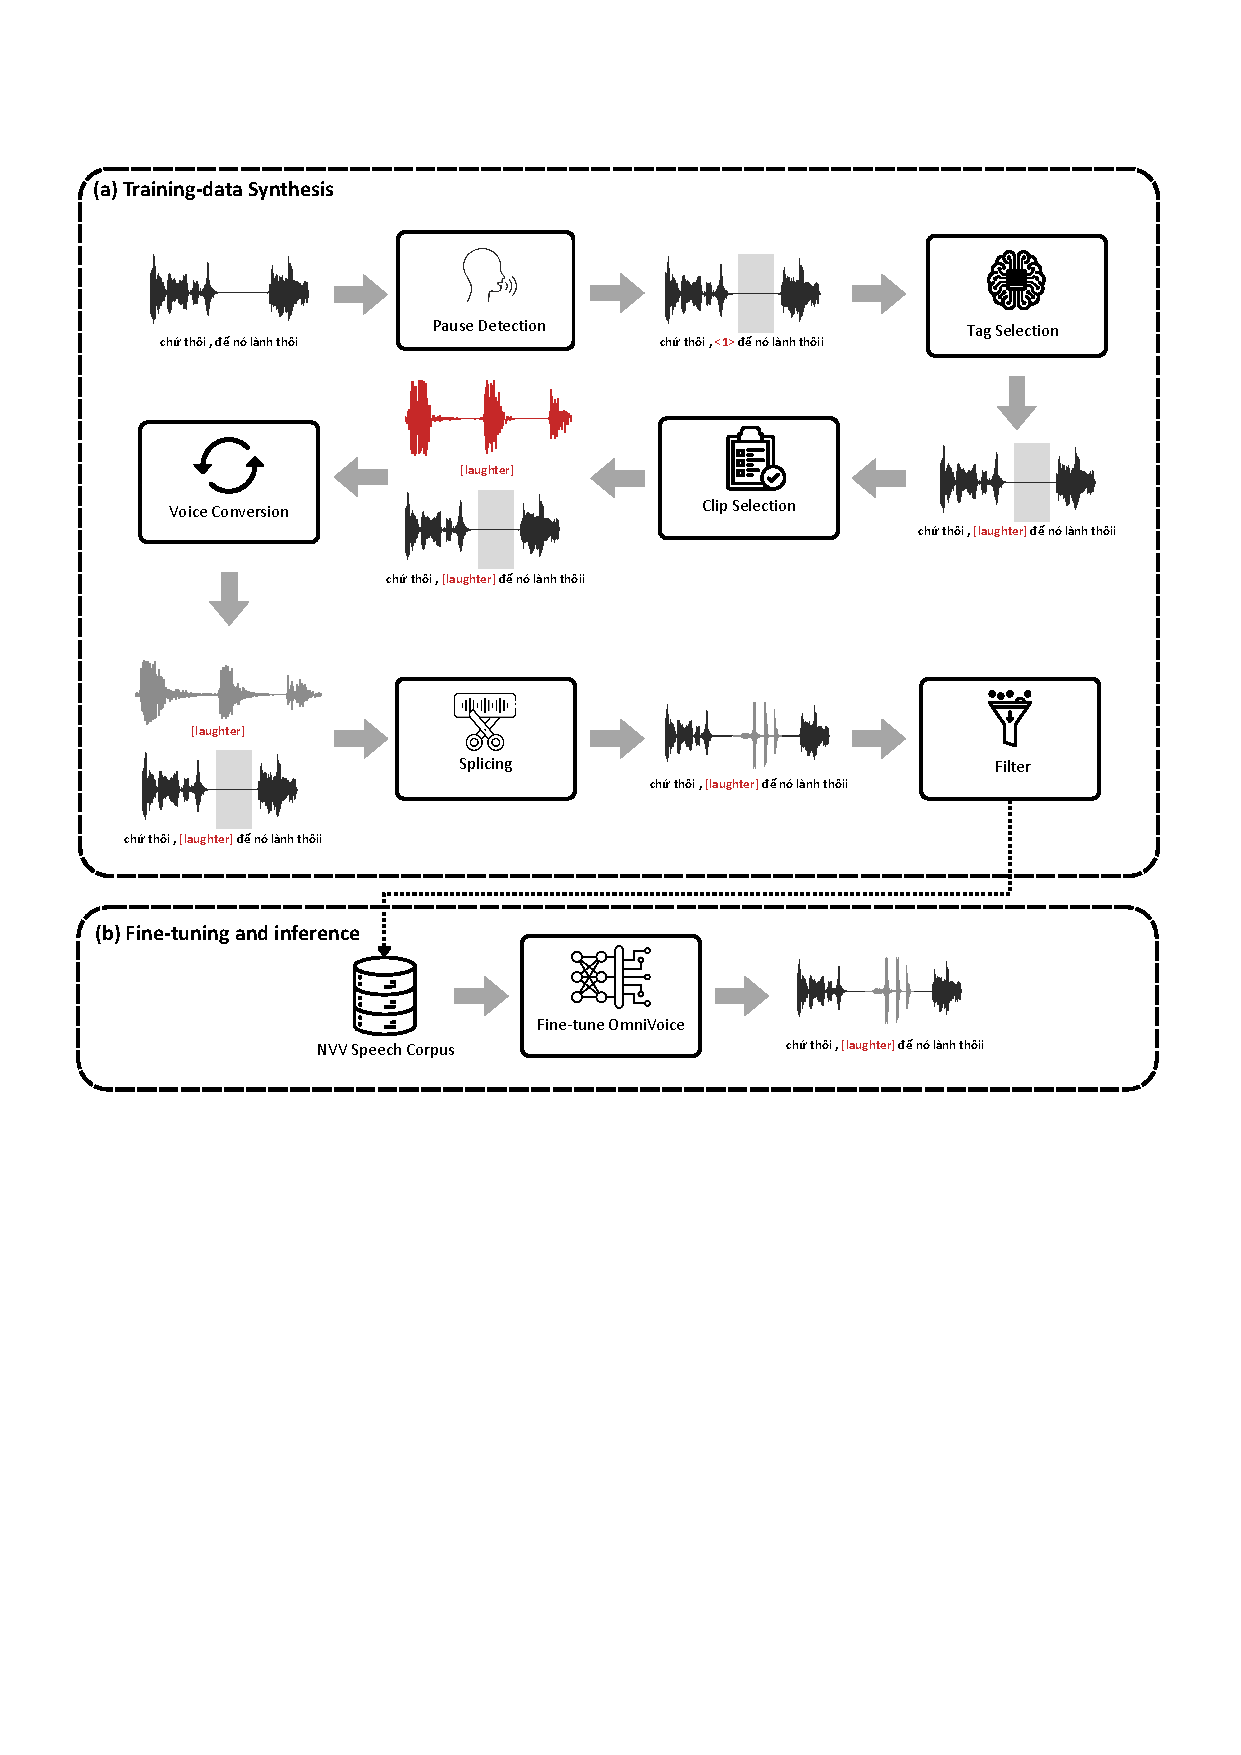
\includegraphics[width=\textwidth, trim=34.8bp 316.7bp 36.8bp 78bp, clip]{figures/overview_canva.pdf}
  \caption{Overview. (a) Training-data synthesis on a real example: pause detection finds the
  pauses between words and marks them in the transcript; tag selection picks one of them and a
  tag, here [laughter]; clip selection draws a laughter clip that suits the speaker; voice
  conversion turns it into the speaker's voice; splicing inserts it into the pause; and the
  filter keeps the result only if its quality holds. (b) The resulting NVV speech corpus is used
  to fine-tune OmniVoice.}
  \label{fig:overview}
\end{figure*}

% Full-width floats appear at the top of the page after the one they are defined on, so
% each table is defined a page ahead of the text that discusses it.
\begin{table*}[t]
\caption{Synthetic NVV training set per tag, after quality filtering.}
\label{tab:synth}
\centering
% Synthetic NVV training set per tag (Table~\ref{tab:synth}). The paper includes it with
% % Synthetic NVV training set per tag (Table~\ref{tab:synth}). The paper includes it with
% % Synthetic NVV training set per tag (Table~\ref{tab:synth}). The paper includes it with
% \input{tables/synth_train} inside a table environment that holds the caption and label.
% Preview: pdflatex synth_train_preview.tex (in this directory).
% Two blocks side by side to keep the table short: the six VocalSound classes on the left, the
% eight added classes on the right.
\small
% Fill from the exported manifest (para-synth export): group rows by the [tag] in `text`,
% count them and sum `duration`, which is re-measured after splicing.
\begin{tabular}{lrrclrr}
\toprule
Tag & Utterances & Hours & & Tag & Utterances & Hours \\
\cmidrule(lr){1-3}\cmidrule(lr){5-7}
\texttt{laughter}       & XX & XX & & \texttt{breathing} & XX & XX \\
\texttt{sigh}           & XX & XX & & \texttt{screaming} & XX & XX \\
\texttt{cough}          & XX & XX & & \texttt{gasp}      & XX & XX \\
\texttt{throatclearing} & XX & XX & & \texttt{snoring}   & XX & XX \\
\texttt{sneeze}         & XX & XX & & \texttt{crying}    & XX & XX \\
\texttt{sniff}          & XX & XX & & \texttt{yawn}      & XX & XX \\
                        &    &    & & \texttt{moan}      & XX & XX \\
                        &    &    & & \texttt{pant}      & XX & XX \\
\midrule
Total                   & XX & XX & & & & \\
\bottomrule
\end{tabular}
 inside a table environment that holds the caption and label.
% Preview: pdflatex synth_train_preview.tex (in this directory).
% Two blocks side by side to keep the table short: the six VocalSound classes on the left, the
% eight added classes on the right.
\small
% Fill from the exported manifest (para-synth export): group rows by the [tag] in `text`,
% count them and sum `duration`, which is re-measured after splicing.
\begin{tabular}{lrrclrr}
\toprule
Tag & Utterances & Hours & & Tag & Utterances & Hours \\
\cmidrule(lr){1-3}\cmidrule(lr){5-7}
\texttt{laughter}       & XX & XX & & \texttt{breathing} & XX & XX \\
\texttt{sigh}           & XX & XX & & \texttt{screaming} & XX & XX \\
\texttt{cough}          & XX & XX & & \texttt{gasp}      & XX & XX \\
\texttt{throatclearing} & XX & XX & & \texttt{snoring}   & XX & XX \\
\texttt{sneeze}         & XX & XX & & \texttt{crying}    & XX & XX \\
\texttt{sniff}          & XX & XX & & \texttt{yawn}      & XX & XX \\
                        &    &    & & \texttt{moan}      & XX & XX \\
                        &    &    & & \texttt{pant}      & XX & XX \\
\midrule
Total                   & XX & XX & & & & \\
\bottomrule
\end{tabular}
 inside a table environment that holds the caption and label.
% Preview: pdflatex synth_train_preview.tex (in this directory).
% Two blocks side by side to keep the table short: the six VocalSound classes on the left, the
% eight added classes on the right.
\small
% Fill from the exported manifest (para-synth export): group rows by the [tag] in `text`,
% count them and sum `duration`, which is re-measured after splicing.
\begin{tabular}{lrrclrr}
\toprule
Tag & Utterances & Hours & & Tag & Utterances & Hours \\
\cmidrule(lr){1-3}\cmidrule(lr){5-7}
\texttt{laughter}       & XX & XX & & \texttt{breathing} & XX & XX \\
\texttt{sigh}           & XX & XX & & \texttt{screaming} & XX & XX \\
\texttt{cough}          & XX & XX & & \texttt{gasp}      & XX & XX \\
\texttt{throatclearing} & XX & XX & & \texttt{snoring}   & XX & XX \\
\texttt{sneeze}         & XX & XX & & \texttt{crying}    & XX & XX \\
\texttt{sniff}          & XX & XX & & \texttt{yawn}      & XX & XX \\
                        &    &    & & \texttt{moan}      & XX & XX \\
                        &    &    & & \texttt{pant}      & XX & XX \\
\midrule
Total                   & XX & XX & & & & \\
\bottomrule
\end{tabular}

\end{table*}


\subsection{Training-data synthesis}\label{sec:data}
Each training example is a real Vietnamese utterance with one NVV spliced into one of its pauses
and a tag inserted at the same point in its transcript. It is built from a pool of NVV clips,
collected once, in six steps per utterance.
\begin{itemize}
\item \textbf{NVV clips.} VocalSound~\citep{vocalsound} alone covers only six classes, and its
  crowdsourced clips often carry long silences or stray speech. We therefore pool clips from
  other NVV corpora and from events cut out of a tagged speech corpus, 17 classes in all
  against SynParaSpeech's 6. Every event is kept only if a sound event detector confirms its
  class, no speech overlaps it, its length is plausible and it is neither noisy nor clipped.
\item \textbf{Pause detection.} Following SynParaSpeech, we first find the pauses where an NVV
  could go and only then let a model choose among them, since placing the tag first fails on
  connected speech. A voice activity detector finds the pauses, a forced aligner the word
  boundaries, and a pause between two words becomes a numbered slot in the transcript, e.g.
  ``chứ thôi , <1> để nó lành thôi''.
\item \textbf{Tag selection.} An omni-modal LLM listens to the recording, reads the marked
  transcript, and picks the slot where a sound would most plausibly occur and the tag that fits,
  where SynParaSpeech uses a text-only model. The tag is inserted in code, so text and audio
  refer to the same point, and a tag balancer withholds any tag that holds too large a share.
\item \textbf{Clip selection.} A clip is drawn at random, weighted towards clips that match the
  speaker on what voice conversion leaves unchanged: intensity, recording clarity, tempo
  (laughter only) and energy tilt, where SynParaSpeech picks one at random. With each distance
  $d_a$ normalised and weighted by $\lambda_a$, a clip is drawn with probability proportional to
  $w = \exp(-\sum_a \lambda_a d_a)$, so a soft-spoken speaker still sometimes gets a loud laugh.
\item \textbf{Voice conversion.} Seed-VC converts the clip into the speaker's voice, using the
  utterance itself as the reference, with pitch conditioning off.
\item \textbf{Splicing.} The event is set to the loudness of the speech before the cut, with a
  per-class offset, and inserted with short exponential fades. Each side gets the target
  silence $T = \bar{T}_p\, s_g\, s^{(c)}$, where $\bar{T}_p$ is the speaker's median pause and
  $s_g$ and $s^{(c)}$ are global and per-class scales; silence is only added, filled with the
  recording's own background noise. SynParaSpeech does not describe this step.
\item \textbf{Filter.} NISQA~\citep{nisqa} scores both the source and the spliced recording, and
  an example is kept only if neither its quality nor its continuity drops past a threshold,
  where SynParaSpeech relies on manual review.
\end{itemize}

\subsection{Fine-tuning and inference}\label{sec:adapt}
OmniVoice~\citep{omnivoice} is a massively multilingual zero-shot TTS model that maps text to
multi-codebook acoustic tokens with a non-autoregressive diffusion language model and clones a
voice from a reference recording. As released, it cannot generate Vietnamese NVVs, for three
reasons. Its tag set is small: only two of its inline tags, [laughter] and [sigh], are
non-verbal sounds, so 15 of our 17 classes have no tag. It has never seen a tag in Vietnamese:
its tagged data come from Chinese and English corpora. And it was not trained for tag control,
which its paper does not evaluate. We therefore fine-tune it on our synthetic data alone, which
supplies all 17 tags on Vietnamese speech. No untagged speech is mixed in: each utterance is
long and carries a single tag, so most of it is ordinary speech, and the same data teaches both
the tags and plain synthesis. The training objective is OmniVoice's own, and at inference the tag is
written inline in the input text.

\section{Experimental Setup}\label{sec:exp}
\begin{table*}[t]
\caption{Zero-shot Vietnamese TTS on the same 238 plain-text utterances. WER in \%. Fish Audio
is queried through an API served with vLLM, not run as a local model, so its RTF is not
measured.}
\label{tab:zeroshot}
\centering
% Zero-shot Vietnamese TTS table body (Table~\ref{tab:zeroshot}). The paper includes it with
% % Zero-shot Vietnamese TTS table body (Table~\ref{tab:zeroshot}). The paper includes it with
% % Zero-shot Vietnamese TTS table body (Table~\ref{tab:zeroshot}). The paper includes it with
% \input{tables/zeroshot} inside a table environment that holds the caption and label.
% Preview: pdflatex zeroshot_preview.tex (in this directory).
% The first four rows, RTF included, are as reported by [CITE]. RTF depends on the hardware:
% measure ours on the same GPU as [CITE], or the RTF column does not compare.
% Released row: VLSP/nvv14_eval.py, task "plain" (text_plain of eval/nvv_test_vi.jsonl x 7 reference voices,
% 2,940 items), report in VLSP/exp/nvv14/report.md. WER over all items (2.48 without the 21 sentences that
% contain digits). RTF on one RTX 5070 Ti, batch of one, float16, 100 items after a warm-up call.
\small
\begin{tabular}{lrrrr}
\toprule
System & MOS $\uparrow$ & WER $\downarrow$ & SS $\uparrow$ & RTF $\downarrow$ \\
\midrule
viXTTS                       & 2.51 & 3.27 & 0.7021 & 0.67 \\
F5-TTS                       & 3.93 & 3.02 & 0.8196 & 0.47 \\
VietVoice-TTS                & 3.58 & 2.37 & 0.7834 & 0.47 \\
VieNeu-TTS                   & 3.69 & 2.00 & 0.6524 & 0.89 \\
\midrule
OmniVoice (released)         & XX{\scriptsize$\pm$XX} & 3.76 & 0.7491 & 0.19 \\
OmniVoice fine-tuned (ours)  & XX{\scriptsize$\pm$XX} & XX & XX & XX \\
\bottomrule
\end{tabular}
 inside a table environment that holds the caption and label.
% Preview: pdflatex zeroshot_preview.tex (in this directory).
% The first four rows, RTF included, are as reported by [CITE]. RTF depends on the hardware:
% measure ours on the same GPU as [CITE], or the RTF column does not compare.
% Released row: VLSP/nvv14_eval.py, task "plain" (text_plain of eval/nvv_test_vi.jsonl x 7 reference voices,
% 2,940 items), report in VLSP/exp/nvv14/report.md. WER over all items (2.48 without the 21 sentences that
% contain digits). RTF on one RTX 5070 Ti, batch of one, float16, 100 items after a warm-up call.
\small
\begin{tabular}{lrrrr}
\toprule
System & MOS $\uparrow$ & WER $\downarrow$ & SS $\uparrow$ & RTF $\downarrow$ \\
\midrule
viXTTS                       & 2.51 & 3.27 & 0.7021 & 0.67 \\
F5-TTS                       & 3.93 & 3.02 & 0.8196 & 0.47 \\
VietVoice-TTS                & 3.58 & 2.37 & 0.7834 & 0.47 \\
VieNeu-TTS                   & 3.69 & 2.00 & 0.6524 & 0.89 \\
\midrule
OmniVoice (released)         & XX{\scriptsize$\pm$XX} & 3.76 & 0.7491 & 0.19 \\
OmniVoice fine-tuned (ours)  & XX{\scriptsize$\pm$XX} & XX & XX & XX \\
\bottomrule
\end{tabular}
 inside a table environment that holds the caption and label.
% Preview: pdflatex zeroshot_preview.tex (in this directory).
% The first four rows, RTF included, are as reported by [CITE]. RTF depends on the hardware:
% measure ours on the same GPU as [CITE], or the RTF column does not compare.
% Released row: VLSP/nvv14_eval.py, task "plain" (text_plain of eval/nvv_test_vi.jsonl x 7 reference voices,
% 2,940 items), report in VLSP/exp/nvv14/report.md. WER over all items (2.48 without the 21 sentences that
% contain digits). RTF on one RTX 5070 Ti, batch of one, float16, 100 items after a warm-up call.
\small
\begin{tabular}{lrrrr}
\toprule
System & MOS $\uparrow$ & WER $\downarrow$ & SS $\uparrow$ & RTF $\downarrow$ \\
\midrule
viXTTS                       & 2.51 & 3.27 & 0.7021 & 0.67 \\
F5-TTS                       & 3.93 & 3.02 & 0.8196 & 0.47 \\
VietVoice-TTS                & 3.58 & 2.37 & 0.7834 & 0.47 \\
VieNeu-TTS                   & 3.69 & 2.00 & 0.6524 & 0.89 \\
\midrule
OmniVoice (released)         & XX{\scriptsize$\pm$XX} & 3.76 & 0.7491 & 0.19 \\
OmniVoice fine-tuned (ours)  & XX{\scriptsize$\pm$XX} & XX & XX & XX \\
\bottomrule
\end{tabular}

\end{table*}


\begin{table*}[h]
\caption{Vietnamese NVV synthesis over 2,940 tagged items (14 classes). Fish Audio is evaluated
on a 280-item subset, through an API served with vLLM, so its RTF is not measured. WER in \%.}
\label{tab:para}
\centering
% NVV synthesis table body (Table~\ref{tab:para}). The paper includes it with
% % NVV synthesis table body (Table~\ref{tab:para}). The paper includes it with
% % NVV synthesis table body (Table~\ref{tab:para}). The paper includes it with
% \input{tables/para_nvv} inside a table environment that holds the caption and label.
% Preview: pdflatex para_nvv_preview.tex (in this directory).
% Released row: VLSP/nvv14_eval.py on eval/nvv_test_vi.jsonl x 7 reference voices (2,940 items), report in
% VLSP/exp/nvv14/report.md. WER over all items (6.94 without the 21 sentences that contain digits). RTF on one
% RTX 5070 Ti, batch of one, float16, 100 items after a warm-up call.
\small
\setlength{\tabcolsep}{5pt}
\begin{tabular}{lrrrrrrrr}
\toprule
 & \multicolumn{2}{c}{NVMR $\downarrow$} & \multicolumn{2}{c}{NVPA $\uparrow$} & & & & \\
\cmidrule(lr){2-3}\cmidrule(lr){4-5}
System & Shared & New & Shared & New & MOS $\uparrow$ & WER $\downarrow$ & SS $\uparrow$ & RTF $\downarrow$ \\
\midrule
OmniVoice (released)         & 0.37 & 0.69 & 0.40 & 0.07 & XX{\scriptsize$\pm$XX} & 8.11 & 0.7539 & 0.17 \\
OmniVoice fine-tuned (ours)  & & & & & XX{\scriptsize$\pm$XX} & XX & XX & XX \\
\bottomrule
\end{tabular}
 inside a table environment that holds the caption and label.
% Preview: pdflatex para_nvv_preview.tex (in this directory).
% Released row: VLSP/nvv14_eval.py on eval/nvv_test_vi.jsonl x 7 reference voices (2,940 items), report in
% VLSP/exp/nvv14/report.md. WER over all items (6.94 without the 21 sentences that contain digits). RTF on one
% RTX 5070 Ti, batch of one, float16, 100 items after a warm-up call.
\small
\setlength{\tabcolsep}{5pt}
\begin{tabular}{lrrrrrrrr}
\toprule
 & \multicolumn{2}{c}{NVMR $\downarrow$} & \multicolumn{2}{c}{NVPA $\uparrow$} & & & & \\
\cmidrule(lr){2-3}\cmidrule(lr){4-5}
System & Shared & New & Shared & New & MOS $\uparrow$ & WER $\downarrow$ & SS $\uparrow$ & RTF $\downarrow$ \\
\midrule
OmniVoice (released)         & 0.37 & 0.69 & 0.40 & 0.07 & XX{\scriptsize$\pm$XX} & 8.11 & 0.7539 & 0.17 \\
OmniVoice fine-tuned (ours)  & & & & & XX{\scriptsize$\pm$XX} & XX & XX & XX \\
\bottomrule
\end{tabular}
 inside a table environment that holds the caption and label.
% Preview: pdflatex para_nvv_preview.tex (in this directory).
% Released row: VLSP/nvv14_eval.py on eval/nvv_test_vi.jsonl x 7 reference voices (2,940 items), report in
% VLSP/exp/nvv14/report.md. WER over all items (6.94 without the 21 sentences that contain digits). RTF on one
% RTX 5070 Ti, batch of one, float16, 100 items after a warm-up call.
\small
\setlength{\tabcolsep}{5pt}
\begin{tabular}{lrrrrrrrr}
\toprule
 & \multicolumn{2}{c}{NVMR $\downarrow$} & \multicolumn{2}{c}{NVPA $\uparrow$} & & & & \\
\cmidrule(lr){2-3}\cmidrule(lr){4-5}
System & Shared & New & Shared & New & MOS $\uparrow$ & WER $\downarrow$ & SS $\uparrow$ & RTF $\downarrow$ \\
\midrule
OmniVoice (released)         & 0.37 & 0.69 & 0.40 & 0.07 & XX{\scriptsize$\pm$XX} & 8.11 & 0.7539 & 0.17 \\
OmniVoice fine-tuned (ours)  & & & & & XX{\scriptsize$\pm$XX} & XX & XX & XX \\
\bottomrule
\end{tabular}

\end{table*}

\begin{table*}[h]
\caption{Listening test on NVV synthesis (1--5, with 95\% confidence intervals).}
\label{tab:mos}
\centering
% Listening-test table body (Table~\ref{tab:mos}). The paper includes it with
% % Listening-test table body (Table~\ref{tab:mos}). The paper includes it with
% % Listening-test table body (Table~\ref{tab:mos}). The paper includes it with
% \input{tables/mos} inside a table environment that holds the caption and label.
% Preview: pdflatex mos_preview.tex (in this directory).
% NVV synthesis only. Each cell is a mean on the 1--5 scale with its 95% confidence interval,
% both to 2 decimals. Ten listeners each rated 40 samples, balanced across the three systems.
% Source values (Fish Audio is run "drama3"):
% base 3.63 +- 0.026, 2.19 +- 0.042, 1.56 +- 0.034; Fish Audio 3.38 +- 0.038, 2.12 +- 0.050,
% 1.96 +- 0.041; fine-tuned 3.89 +- 0.012, 3.15 +- 0.044, 2.96 +- 0.046.
\small
\begin{tabular}{lccc}
\toprule
System & \textbf{MOS-Q} $\uparrow$ & \textbf{MOS-N} $\uparrow$ & \textbf{MOS-E} $\uparrow$ \\
\midrule
Fish Audio                   & 3.38 $\pm$ 0.04 & 2.12 $\pm$ 0.05 & 1.96 $\pm$ 0.04 \\
OmniVoice                   & & & \\
\quad + base                 & 3.63 $\pm$ 0.03 & 2.19 $\pm$ 0.04 & 1.56 $\pm$ 0.03 \\
\quad + fine-tuned (ours)    & 3.89 $\pm$ 0.01 & 3.15 $\pm$ 0.04 & 2.96 $\pm$ 0.05 \\
\bottomrule
\end{tabular}
 inside a table environment that holds the caption and label.
% Preview: pdflatex mos_preview.tex (in this directory).
% NVV synthesis only. Each cell is a mean on the 1--5 scale with its 95% confidence interval,
% both to 2 decimals. Ten listeners each rated 40 samples, balanced across the three systems.
% Source values (Fish Audio is run "drama3"):
% base 3.63 +- 0.026, 2.19 +- 0.042, 1.56 +- 0.034; Fish Audio 3.38 +- 0.038, 2.12 +- 0.050,
% 1.96 +- 0.041; fine-tuned 3.89 +- 0.012, 3.15 +- 0.044, 2.96 +- 0.046.
\small
\begin{tabular}{lccc}
\toprule
System & \textbf{MOS-Q} $\uparrow$ & \textbf{MOS-N} $\uparrow$ & \textbf{MOS-E} $\uparrow$ \\
\midrule
Fish Audio                   & 3.38 $\pm$ 0.04 & 2.12 $\pm$ 0.05 & 1.96 $\pm$ 0.04 \\
OmniVoice                   & & & \\
\quad + base                 & 3.63 $\pm$ 0.03 & 2.19 $\pm$ 0.04 & 1.56 $\pm$ 0.03 \\
\quad + fine-tuned (ours)    & 3.89 $\pm$ 0.01 & 3.15 $\pm$ 0.04 & 2.96 $\pm$ 0.05 \\
\bottomrule
\end{tabular}
 inside a table environment that holds the caption and label.
% Preview: pdflatex mos_preview.tex (in this directory).
% NVV synthesis only. Each cell is a mean on the 1--5 scale with its 95% confidence interval,
% both to 2 decimals. Ten listeners each rated 40 samples, balanced across the three systems.
% Source values (Fish Audio is run "drama3"):
% base 3.63 +- 0.026, 2.19 +- 0.042, 1.56 +- 0.034; Fish Audio 3.38 +- 0.038, 2.12 +- 0.050,
% 1.96 +- 0.041; fine-tuned 3.89 +- 0.012, 3.15 +- 0.044, 2.96 +- 0.046.
\small
\begin{tabular}{lccc}
\toprule
System & \textbf{MOS-Q} $\uparrow$ & \textbf{MOS-N} $\uparrow$ & \textbf{MOS-E} $\uparrow$ \\
\midrule
Fish Audio                   & 3.38 $\pm$ 0.04 & 2.12 $\pm$ 0.05 & 1.96 $\pm$ 0.04 \\
OmniVoice                   & & & \\
\quad + base                 & 3.63 $\pm$ 0.03 & 2.19 $\pm$ 0.04 & 1.56 $\pm$ 0.03 \\
\quad + fine-tuned (ours)    & 3.89 $\pm$ 0.01 & 3.15 $\pm$ 0.04 & 2.96 $\pm$ 0.05 \\
\bottomrule
\end{tabular}

\end{table*}



\subsection{Data}
Training uses only the synthetic NVV set, built from ViVoice~\citep{vivoice}: 224,064
utterances (810.8\,h), each with one event, with 10,190 to 13,522 utterances per tag
(Table~\ref{tab:synth}).

\subsection{Training}
We initialise from the public OmniVoice checkpoint and fine-tune all parameters with the
default settings of OmniVoice's training configuration for 10,000 steps, on NVIDIA B200 GPUs.

\subsection{Baselines}
We evaluate two tasks. In zero-shot TTS, the input is plain Vietnamese text without tags; this
task checks that fine-tuning keeps ordinary synthesis intact. Its baselines are the released
OmniVoice, four Vietnamese TTS systems (viXTTS, F5-TTS, VietVoice-TTS and VieNeu-TTS) and Fish
Audio's TTS, queried through an API served with vLLM. In NVV synthesis, the input is tagged text, and each tag must
become the matching vocalization at its position; its baselines are the released OmniVoice and
Fish Audio. The listening test covers Fish Audio and both OmniVoice models.

\subsection{Evaluation}
For zero-shot TTS, every system is evaluated on the same 238 utterances sampled from VietVoice,
an internal Vietnamese speech dataset. For NVV synthesis, we use 420 real Vietnamese sentences,
30 for each of 14 classes, each chosen so that the tag fits its content; each is synthesised
with 7 reference voices that are not in the training data, giving 2,940 items per system. For
both OmniVoice models we tokenise the whole tagged string at inference, as in training.

NV placement accuracy (NVPA, 0--1, higher is better) is the share of tags for which a sound
event detector finds a vocalization of the tagged class at the tag's position. The NV miss rate
(NVMR, 0--1, lower is better) is the share of tags with no vocalization at all. Word error rate
(WER, in \%, lower is better) compares a Vietnamese ASR transcript of the output with the input
text. SIM-o (0--1, higher is better) is the cosine between the speaker embeddings of the output
and of the reference voice. The real-time factor (RTF, lower is better) is the time to
synthesise an utterance divided by its duration, on one NVIDIA A100 GPU. In the listening test,
ten native Vietnamese listeners each rate 40 NVV samples, balanced across the three systems,
from 1 (bad) to 5 (excellent) on quality
(MOS-Q), naturalness (MOS-N) and expressiveness (MOS-E), the last asking whether the
vocalization is the one the tag asks for and carries the feeling of the sentence.

\section{Results}\label{sec:results}
Given Vietnamese text, the released OmniVoice produces no vocalization at 37\% of the [laughter]
and [sigh] tags, the two it supports, and at 69\% of the other 12; even its own two tags behave
very differently, with a correct laugh for 79\% of [laughter] tags but a correct sigh for only
1\% of [sigh] tags. Fine-tuning on our data changes this (Table~\ref{tab:para}). The share of
missed tags falls from 64\% to 35\%, and the share realised correctly rises from 11.5\% to 50\%:
from 40\% to 86\% on laughter and sigh and from 7\% to 44\% on the new tags. The word error
rate on the tagged sentences also falls, from 8.11\% to 6.73\%, and speaker similarity stays
close (0.74 against 0.75). On plain text (Table~\ref{tab:zeroshot}), the cost is small: the word
error rate rises from 3.93\% to 4.78\%, speaker similarity is 0.84 for both models, and the RTF
stays at 0.06. Fish Audio does worse than our model on both tasks: a word error rate of
11.31\% on plain text and, on NVV synthesis, 65\% of tags missed and 23\% correct. Its high
word error rate (60.48\%) and low speaker similarity (0.32) on NVV synthesis share one cause:
after a tag, whether or not it produced the sound, Fish Audio often drops the rest of the
sentence and leaves a long pause in its place.
Listeners prefer the fine-tuned model on all three scores (Table~\ref{tab:mos}). Its
naturalness rises from 2.19 to 3.15 and its expressiveness from 1.56 to 2.96, against 2.12 and
1.96 for Fish Audio, and its audio quality is the highest of the three (3.89, against 3.63 and
3.38).

\section{Conclusion}\label{sec:conclusion}
We set out to give Vietnamese TTS the ability to laugh, sigh, cough and make other non-verbal
sounds where the text asks for them. We built a pipeline that creates the missing training data
automatically from real Vietnamese speech, producing about 811 hours over 17 sound types.
Fine-tuned on this data, OmniVoice makes the right sound at the right place for 50\% of tags instead of 11.5\%,
misses 35\% instead of 64\%, and reads tagged sentences more accurately, at a small cost on plain
text and with a real-time factor of 0.06; listeners rate its naturalness and expressiveness well
above both the released model and Fish Audio.

The work has limits. Each training example carries one sound, inserted into an existing pause,
so sounds that overlap speech, such as laughing while talking, are not covered. The inserted
sounds are recorded by other people and only converted into the target voice. Burp, grunt and
yell are trained but not yet tested. Next, we plan to train a version on ViVoice alone to separate the effect of the NVV data from that of extra Vietnamese
training, and to extend the test set to all 17 sound types.

\bibliographystyle{unsrtnat}
\bibliography{iclr2025_conference}

\end{document}
